\documentclass[12pt]{article}
\usepackage{geometry}
\usepackage{amsmath, amsfonts, amssymb}
\usepackage[utf8]{inputenc}
\usepackage{graphicx}
\usepackage[round]{natbib}
\usepackage{subfig}
\usepackage{hyperref}
\usepackage{physics}
\usepackage{float}
\usepackage{cancel}


\hypersetup{
	bookmarksopen=true,
	colorlinks=true,
	linkcolor=blue,
	citecolor=blue,
	urlcolor=black,	
	linktoc=all,
	pdftitle={Waves in Cosserat media},
	pdfauthor={N. Guarin-Zapata, J. Gomez},
	pdfkeywords={Finite element method, Cosserat solids, Bloch theorem, Wave propagation},
	pdfsubject={Elastodynamics},
	pdfpagemode=UseOutlines,
	pdfstartview=FitH}


\title{\textbf{The micropolar continuum theory: a revision from the wave propagation perspective}}

\author{Gary Dargush \and Ali Reza Hadjesfandiari \and Nicolás Guarín-Zapata \and Juan Gomez}


\begin{document}
\maketitle

\section{Introduction}
The classical model of continuum mechanics lacks a length scale thus it is unable to capture so-called size effects. In the early 1900s, starting with the work from the Cosserat brothers \citep{Cosserat1909} a series of non-classical models were proposed with an intrinsic capability to account for microstructural effects while retaining a continuum approach. Broadly speaking these models could be categorized into micropolar models incorporating additional degrees of freedom and reduced or gradient models keeping additional displacement gradients in its kinematic formulation. Although most of these formulations are mathematically consistent and are also able to predict numerical results valid under particular scenarios, not all of them are fully consistent as a continuum theory. For instance in a series of recent contribution Hadjesfandiari and Dargush() and Dargush and Hadjesfandiari() presented arguments questioning the continuum mechanics consistency of non-classical models. Moreover, these authors (see Hadjesfandiari and Dargush() ) formulated a valid Couple stress framework after fixing the kinematical indeterminacy in the reduced couple stress theory.

Among the non-classical models, the micropolar theory \citep{Eringen1966} is very convenient since it just introduces an additional rotation independent of the macro-rotation which conserves the original structure of the displacements equations from classical theory and also eliminates compatibility issues in the corresponding numerical implementations. In this work we conduct additional scrutiny o the micropolar model but examining it from the point of view of its response under dynamic conditions and particularly from its wave propagation perspective. We start by reviewing the stress and displacement equations of motion and in general the mathematical consistency of the problem. Using vector potentials we find the existent propagation modes, derive dispersion relations and reflection coefficients. As a final verification we use Bloch analysis to obtain the band structure of a homogeneous micropolar model.



\section{Fundamental relationships}
\subsection{Conservation of linear and angular momentum}
In micropolar elasticity we have conservation of linear and angular momentum given by the following expressions
\begin{subequations}\label{eq:conservation}
  \begin{align}
    &\sigma_{ji, i} + f_i = \rho \ddot{u}_i\\
    &\sigma_{jk} \epsilon_{ijk} + \mu_{ji, j} + c_i = J \ddot{\varphi}\, .
  \end{align}
\end{subequations}

\subsection{Kinematic relations}
The (linearized) kinematic relations are given by
\begin{subequations}\label{eq:kinematics}
  \begin{align}
    & \gamma_{ji} = u_{i,j} - \epsilon_{kji} \varphi_k\\
    & \kappa_{ji} = \varphi_{i,j}\, .
  \end{align}
\end{subequations}

\subsection{Constitutive equations}
In the linear regime, the constitutive equations are
\begin{subequations}\label{eq:constitutive}
  \begin{align}
    & \sigma_{ji} = (\mu + \alpha) \gamma_{ji} + (\mu - \alpha) \gamma_{ij} + \lambda \gamma_{kk} \delta_{ij}\\
    & \mu_{ji} = (\gamma + \varepsilon) \kappa_{ji} + (\gamma - \varepsilon) \kappa_{ij} + \beta \kappa_{kk} \delta_{ij}\, .
  \end{align}
\end{subequations}

These constitutive equations can also be written as
\begin{align*}
    & \sigma_{ji} = \mu \gamma_{(ij)} + 2 \alpha \gamma_{[ij]} + \lambda \gamma_{kk} \delta_{ij}\\
    & \mu_{ji} = \gamma \kappa_{(ij)} + 2\varepsilon \kappa_{[ij]} + \beta \kappa_{kk} \delta_{ij}\, ,
\end{align*}
where we have separated the symmetric and antisymmetric parts of the 

\section{Derivation of the equations for displacements and rotations}
We can start writing the conservation equations \eqref{eq:conservation} as kinematic variables using the constitutive equations \eqref{eq:constitutive}, to obtain:
\begin{align*}
 & (\mu + \alpha) \gamma_{ji, j} + (\mu - \alpha) \gamma_{ij,j} + \lambda \gamma_{kk, i} + f_i = \rho \ddot{u}_i\\
  & \epsilon_{ijk}(\mu + \alpha) \gamma_{jk} + \epsilon_{ijk}(\mu - \alpha) \gamma_{kj} + \cancelto{0}{\epsilon_{ijk} \delta_{jk} \lambda \gamma_{rr}} + (\gamma + \epsilon) \kappa_{ji,j} + (\gamma - \epsilon) \kappa_{ij,j} + \beta \kappa_{kk, i} + c_i = J \ddot{\varphi}_i\, .
\end{align*}

Let's focus in the equations for the conservation of linear momentum first. If we replace the kinematics relations, we get
\[(\mu + \alpha) u_{i, jj} - (\mu + \alpha)\epsilon_{kji} \varphi_{k, j} + (\mu - \alpha) u_{j, ij} + (\mu - \alpha)\epsilon_{kji} \varphi_{k,j} + \lambda u_{k,ki} - \cancelto{0}{\epsilon_{krr}\lambda \varphi_{k,j}} + f_i = \rho \ddot{u}_i\, , \]
or
\[(\mu + \alpha) u_{i,jj} + (\mu - \alpha) u_{j,ij} + \lambda u_{k,kj} - 2\alpha \epsilon_{kji} + f_i = \rho \ddot{u}_i\, .\]

And, using the identity \(a_{i,jj} = a_{j,ji} - \epsilon_{ijk} \epsilon_{klm} a_{m,lj}\),
\[(\mu + \alpha) u_{k, ki} - \epsilon_{ijk} \epsilon_{klm} (\mu + \alpha) u_{m, lj} + (\mu - \alpha) u_{j,ij} + \lambda u_{k, ki} - 2\alpha \epsilon_{kji} \varphi_{k,j} + f_i = \rho \ddot{u}_i\, ,\]
grouping \(u_{k,ki}\),
\[(\mu + \alpha + \lambda) u_{k, ki} - \epsilon_{ijk} \epsilon_{klm} (\mu + \alpha) u_{m,lj} + (\mu - \alpha) u_{j, ij} + 2\alpha \epsilon_{ijk} \varphi_{k,j} + f_i = \rho \ddot{u}_i\, ,\]
but \(u_{j, ij} = u_{j, ji}\), thus
\[(\lambda + 2\mu) u_{k, ki} - \epsilon_{ijk} \epsilon_{klm} (\mu + \alpha) u_{m,lj}+ 2\alpha \epsilon_{ijk} \varphi_{k,j} + f_i = \rho \ddot{u}_i\, .\]

Following a similar approach, we obtain
\[(\beta + 2\gamma) \varphi_{k, ki} - \epsilon_{ijk} \epsilon_{klm} (\gamma + \varepsilon) u_{m,lj}+ 2\alpha \epsilon_{ijk} u_{k,j} - 4\alpha\varphi + c_i = J \ddot{\varphi}_i\, ,\]
for rotations.

\section{Equations in index and vector notation}
Authors presents the equations in slightly different ways, in this section we present the equations in two different forms.

One form is
\begin{subequations}
  \begin{align}
    & (\mu + \alpha) u_{i, jj} + (\lambda + \mu - \alpha) u_{j,ji} + 2\alpha \epsilon_{ijk}\varphi_{k,j} + f_i = \rho \ddot{u}_i\, \\
    & (\gamma + \varepsilon) \varphi_{i, jj} + (\beta + \gamma - \varepsilon) \varphi_{j,ji} + 2\alpha \epsilon_{ijk}u_{k,j} - 4\alpha \varphi_i  + c_i = J \ddot{\varphi}_i\, ,
  \end{align}
\end{subequations}
or, in vector notation
\begin{align*}
    & (\mu + \alpha)\laplacian{\vb{u}} + (\lambda + \mu - \alpha) \grad\div\vb{u} + 2\alpha \curl\vb{\varphi} + \vb{f} = \rho \pdv[2]{\vb{u}}{t}\, \\
    & (\gamma + \varepsilon) \laplacian\vb{\varphi} + (\beta + \gamma - \varepsilon) \grad\div\vb{\varphi} + 2\alpha \curl\vb{u} - 4\alpha \vb{\varphi}  + \vb{c} = J \pdv[2]{\varphi}{t}\, .
\end{align*}

We find the second form more appropriated for wave propagation. This one, reads
\begin{subequations}
  \begin{align}
    & (\lambda + 2\mu) u_{k, ki} - \epsilon_{ijk} \epsilon_{klm} (\mu + \alpha) u_{m,lj}+ 2\alpha \epsilon_{ijk} \varphi_{k,j} + f_i = \rho \ddot{u}_i, \\
    & (\beta + 2\gamma) \varphi_{k, ki} - \epsilon_{ijk} \epsilon_{klm} (\gamma + \varepsilon) u_{m,lj}+ 2\alpha \epsilon_{ijk} u_{k,j} - 4\alpha\varphi + c_i = J \ddot{\varphi}_i\, ,
  \end{align}
\end{subequations}
or, in vector notation
\begin{subequations}\label{eq:disp_vector}
  \begin{align}
    & (\lambda + 2\mu) \grad\div\vb{u} - (\mu + \alpha)\curl\curl\vb{u} + 2\alpha \curl\vb{\varphi} + \vb{f} = \rho \pdv[2]{\vb{u}}{t}, \\
    & (\beta + 2\gamma) \grad\div\vb{\varphi} - (\gamma + \varepsilon) \curl\curl\vb{\varphi} +  2\alpha \curl\vb{u} - 4\alpha\vb{\varphi} + \vb{c} = J \pdv[2]{\vb{\varphi}}{t}\, .
  \end{align}
\end{subequations}

\section{Waves in micropolar solids}
Let's write equation \eqref{eq:disp_vector} in a slightly different way, where we regroup the material constants in a different way and neglect body forces
\begin{subequations}
  \begin{align}\label{eq:disp_waves}
    & c_1^2 \grad\div\vb{u} - c_2^2\curl\curl\vb{u} + K^2 \curl\vb{\varphi} =  \pdv[2]{\vb{u}}{t}, \\
    & c_3^2 \grad\div\vb{\varphi} - c_4^2 \curl\curl\vb{\varphi} +  Q^2 \curl\vb{u} - 2Q^2 \vb{\varphi} = \pdv[2]{\vb{\varphi}}{t}\, .
  \end{align}
\end{subequations}
where,
\begin{equation*}
\begin{split}
c_1^2 = \frac{\lambda +2\mu}{\rho},\quad &c_3^2 =\frac{\beta +2\gamma}{J},\\
c_2^2 = \frac{\mu +\alpha}{\rho},\quad &c_4^2 =\frac{\gamma + \varepsilon}{J},\\
K^2= \frac{2\alpha}{\rho},\quad &Q^2 =\frac{2\alpha}{J} \, ,
\end{split}
\end{equation*}


To identify types of propagating waves that can arise in the micropolar medium we expand our main variables in terms of scalar and vector potentials, as follows
\begin{align*}
\vb{u} &= \grad \phi + \curl\vb{\Gamma}\, ,\\
\vb{\varphi} &= \grad \tau + \curl\vb{E}\, ,
\end{align*}
with
\begin{align*}
&\div\vb{\Gamma} = 0\\
&\div\vb{E} = 0\, .
\end{align*}

If we plug these in \eqref{eq:disp_waves}, we obtain the following, after some manipulations,
\begin{subequations}
  \begin{align}\label{eq:potential_waves}
    c_1^2 \laplacian\phi &= \pdv[2]{\phi}{t}\\
    c_3^2 \laplacian\tau - 2Q^2\tau &= \pdv[2]{\tau}{t}\\
    \begin{bmatrix}
      c_2^2\laplacian &K^2\curl\\
      Q^2\curl &c_4^2\laplacian - 2Q^2
    \end{bmatrix}
    \begin{Bmatrix} \vb{\Gamma}\\ \vb{E}\end{Bmatrix} &=
    \pdv[2]{t} \begin{Bmatrix} \vb{\Gamma}\\ \vb{E}\end{Bmatrix}\, ,
  \end{align}
\end{subequations}
where we can see that the equations for the scalar potentials are uncoupled, while the ones
for the vector potentials are coupled.

\subsection{Dispersion relations}
If we assume that the potentials are plane waves we can find the dispersion relations. Particularly, for the coupled waves, we have
\begin{align*}
\vb{\Gamma} &= \vb{A}\exp(i\kappa x - i\omega t)\\
\vb{E} &= \vb{B}\exp(i\kappa x - i\omega t)\, ,
\end{align*}
and plugging it into the coupled equation we end up with the following system of equations
\[\begin{bmatrix}
M_{11} &M_{12}\\
M_{21} &M_{22}\end{bmatrix}
\begin{Bmatrix} \vb{A}\\ \vb{B}\end{Bmatrix}
= \vb{0}\, ,\]
with
\begin{align*}
&M_{11} =
(c_{2}^{2} \kappa^{2} - \omega^{2})
\begin{bmatrix}
1 & 0 & 0\\
0 & 1 & 0 \\
0 & 0 & 1
\end{bmatrix}\\
&M_{12} =
\begin{bmatrix}
0 & 0 & 0\\
0 & 0 & i K^{2} \kappa\\
0 & -i K^{2} \kappa & 0
\end{bmatrix}\\
&M_{21} =
\begin{bmatrix}
0 & 0 & 0 \\
0 & 0 & i Q^{2} \kappa \\
0 & -i Q^{2} \kappa & 0 
\end{bmatrix}\\
&M_{22} =
(2 Q^{2} + c_{4}^{2} \kappa^{2} - \omega^{2})\begin{bmatrix}
1 &0 &0\\
0 &1 &0\\
0 &0 &1
\end{bmatrix}\, .
\end{align*}

Since we are not interested in the null solution, we have
\[\det\begin{bmatrix}
M_{11} &M_{12}\\
M_{21} &M_{22}\end{bmatrix}=0\, ,\]
that leads to the dispersion equation 
\begin{equation*}
\omega^2 = Q^{2} + \frac{c_{2}^{2} \kappa^{2}}{2} + \frac{c_{4}^{2} \kappa^{2}}{2} \mp \frac{1}{2} \sqrt{4 K^{2} Q^{2} \kappa^{2} + 4 Q^{4} - 4 Q^{2} c_{2}^{2} \kappa^{2} + 4 Q^{2} c_{4}^{2} \kappa^{2} + c_{2}^{4} \kappa^{4} - 2 c_{2}^{2} c_{4}^{2} \kappa^{4} + c_{4}^{4} \kappa^{4}}\, ,
\end{equation*}
where the minus signs corresponds to the transverse wave and the plus sign corresponds to the rotational wave.

The dispersion relations are then
\begin{align}
&\omega_P = c_1 \kappa\, ,\\
&\omega_{RL} = \sqrt{2Q^2 + c_3^2 \kappa^2}\, ,\\
&\omega_S = \sqrt{Q^{2} + \frac{(c_2^2 + c_4^2)}{2}\kappa^2 - \frac{1}{2} \sqrt{4Q^4 +
   4Q^2[(c_4^2 - c_2^2) + K^2]\kappa^2 + (c_4^2 - c_2^2)^2 \kappa^4}}\, ,\\
&\omega_{RT} = \sqrt{Q^{2} + \frac{(c_2^2 + c_4^2)}{2}\kappa^2 + \frac{1}{2} \sqrt{4Q^4 +
   4Q^2[(c_4^2 - c_2^2) + K^2]\kappa^2 + (c_4^2 - c_2^2)^2 \kappa^4}}\, ,
\end{align}
where we can see that the only wave that is not dispersive is the P-wave, since the relationship between wavenumber and frequency is linear.

\subsubsection{Wave speeds}
We can write the phase speeds \(v_i \equiv \omega_i/\kappa\), to obtain
\begin{align}
&v_P = c_1 \, ,\\
&v_{RL} = \sqrt{\frac{2Q^2}{\kappa^2} + c_3^2}\, ,\\
&v_S = \sqrt{\frac{Q^2}{\kappa^2} + \frac{(c_2^2 + c_4^2)}{2} - \frac{1}{2} \sqrt{\frac{4Q^4}{\kappa^4} + \frac{4Q^2}{\kappa^2}[(c_4^2 - c_2^2) + K^2] + (c_4^2 - c_2^2)^2}}\, ,\\
&v_{RT} = \sqrt{\frac{Q^2}{\kappa^2} + \frac{(c_2^2 + c_4^2)}{2} + \frac{1}{2} \sqrt{\frac{4Q^4}{\kappa^4} + \frac{4Q^2}{\kappa^2}[(c_4^2 - c_2^2) + K^2] + (c_4^2 - c_2^2)^2}}\, ,
\end{align}
if we take the limit \(\kappa \rightarrow 0\), we obtain
\[\lim_{\kappa \rightarrow 0} v_S = \sqrt{c_2^2 - \frac{K^2}{2}}=\sqrt{\frac{\mu}{\rho}}\, ,\]
that corresponds to the phase speed of the shear wave in classical media. And, if we take the high frequency limit (\(\kappa \rightarrow \infty\)), we find that
\begin{align*}
&\lim_{\kappa \rightarrow \infty}v_{RL} = c_3\, ,\\
&\lim_{\kappa \rightarrow \infty}v_S = c_2\, ,\\
&\lim_{\kappa \rightarrow \infty}v_{RT} = c_4\, .
\end{align*}

We can also compute the group speed \(g_i = \partial \omega_i/\partial \kappa\), to obtain
\begin{align}
&g_P = c_1 \, ,\\
&g_{RL} = \frac{c_3^2 \kappa}{\omega_{RL}}\, ,\\
&g_S = \frac{1}{2\omega_S}\left[(c_2^2 + c_4^2)\kappa - \frac{2Q^2[(c_4^2 - c_2^2) + K^2]\kappa + (c_4^2 + c_2^2)^2\kappa^3}{\sqrt{4Q^4 + 4Q^2[(c_4^2 - c_2^2) + K^2]\kappa^2 + (c_4^2 - c_2^2)^2 \kappa^4}}\right] \, ,\\
&g_{RT} = \frac{1}{2\omega_{RT}}\left[(c_2^2 + c_4^2)\kappa + \frac{2Q^2[(c_4^2 - c_2^2) + K^2]\kappa + (c_4^2 + c_2^2)^2\kappa^3}{\sqrt{4Q^4 +  4Q^2[(c_4^2 - c_2^2) + K^2]\kappa^2 + (c_4^2 - c_2^2)^2 \kappa^4}}\right]\, ,
\end{align}
if we take the limit \(\kappa \rightarrow 0\), we obtain
\begin{align*}
&\lim_{\kappa \rightarrow 0}g_{RL} = 0\, ,\\
&\lim_{\kappa \rightarrow 0}g_S = \lim_{\kappa \rightarrow 0} v_S = \sqrt{c_2^2 - \frac{K^2}{2}}=\sqrt{\frac{\mu}{\rho}}\, ,\\
&\lim_{\kappa \rightarrow 0}g_{RT} = 0\, .
\end{align*}

And in the high frequency limit (\(\kappa \rightarrow \infty\)), we find that
\begin{align*}
&\lim_{\kappa \rightarrow \infty}g_{RL} = \lim_{\kappa \rightarrow \infty}v_{RL} = c_3\, ,\\
&\lim_{\kappa \rightarrow \infty}g_S = \lim_{\kappa \rightarrow \infty}v_S = c_2\, ,\\
&\lim_{\kappa \rightarrow \infty}g_{RT} = \lim_{\kappa \rightarrow \infty}v_{RT} = c_4\, .
\end{align*}

\subsubsection{Dispersion relations as functions of frequency}
In some applications is useful to have the dispersion relations as functions of frequency instead of wavenumber. In this case they are given by
\begin{align}
&\kappa_P = \frac{\omega}{c_1}\, ,\\
&\kappa_{RL} = \frac{\sqrt{\omega^2 - 2Q^2}}{c_3}\, ,\\
&\kappa_S = \sqrt{\frac{D\omega^2}{2} + \frac{1}{2} \sqrt{D^2 \omega^4 - 4E\omega^4}}\, ,\\
&\kappa_{RT} = \sqrt{\frac{D\omega^2}{2} - \frac{1}{2} \sqrt{D^2 \omega^4 - 4E\omega^4}}\, ,
\end{align}
with
\begin{align*}
&D = \frac{2Q^2}{\omega^2 c_4^2} - \frac{K^2 Q^2}{c_2^2 c_4^2 \omega^2} - \frac{1}{c_2^2} - \frac{1}{c_4^2}\, ,\\
&E = \frac{1}{c_2^2 c_4^2} - \frac{2Q^2}{c_2^2 c_4^2 \omega^2}\, .
\end{align*}

And, equivalently, write the slowness for each wave, namely
\begin{align}
&s_P(\omega) \equiv \frac{1}{v_P(\omega)} = \frac{1}{c_1}\, ,\\
&s_{RL}(\omega) \equiv \frac{1}{v_{RL}(\omega)} = \sqrt{\frac{1}{c_3} - \frac{2Q^2}{\omega^2 c_3^2}}\, ,\\
&s_S(\omega)\equiv \frac{1}{v_S(\omega)} = \sqrt{\frac{D}{2} + \frac{1}{2} \sqrt{D^2 - 4E}}\, ,\\
&s_{RT}(\omega) \equiv \frac{1}{v_{RT}(\omega)} = \sqrt{\frac{D}{2} - \frac{1}{2} \sqrt{D^2 - 4E}}\, .
\end{align}

\subsection{Reflection of a plane wave on a plane boundary}
Let us consider now the problem of a plane boundary, as shown in the following schematic.
\begin{figure}[h]
  \centering
  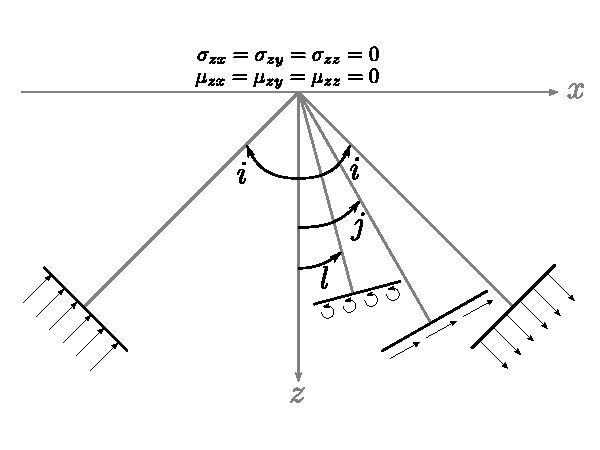
\includegraphics[scale=1]{img/reflection_schematic.pdf}
  \caption{Schematic for analysis of reflected waves set up by a plane P-wave incident on the free surface of a micropolar half-space.}
  \label{fig:reflection_schematic}
\end{figure}

If we consider waves lying on the \(zx\) plane, the equations of motions reduce to
\begin{align*}
&c_1^2\left[\pdv[2]{u_x}{x} + \pdv{u_z}{x}{z}\right] - c_2^2\left[\pdv{u_z}{x}{z} - \pdv[2]{u_x}{z}\right] - K^2\pdv{\phi_y}{z} = \ddot{u_x}\, ,\\
&c_1^2\left[\pdv{u_x}{x}{z} + \pdv[2]{u_z}{z}\right] - c_2^2\left[\pdv{u_x}{x}{z} - \pdv[2]{u_z}{z}\right] + K^2\pdv{\phi_y}{x} = \ddot{u_z}\, ,\\
&Q^2\left[\pdv{u_x}{z} - \pdv{u_z}{x}\right] + c_4^2\left[\pdv[2]{\phi_y}{x} + \pdv[2]{\phi_y}{z}\right] - 2Q^2\phi_y = \ddot{\phi_y}\, .
\end{align*}

And the strain and curvature tensors are
\begin{align*}
&\gamma = \begin{bmatrix}
  \pdv{u_x}{x} &0 &\pdv{u_z}{x} + \phi_y\\
  0 & 0 &0\\
  \pdv{u_x}{z} - \phi_y &0 &\pdv{u_z}{z}
\end{bmatrix}\, ,\\
&\kappa = \begin{bmatrix}
  0 &\pdv{\phi_y}{x} &0\\
  0 &0 &0\\
  0 &\pdv{\phi_y}{z} &0
\end{bmatrix}\, .
\end{align*}

While the force-stress and  couple-stress tensor read
\begin{align*}
&\sigma = \begin{bmatrix}
  (\lambda + 2\mu)\pdv{u_x}{x} + \lambda \pdv{u_x}{z} &0 &(\mu + \alpha)\pdv{u_x}{z} + (\mu - \alpha)\pdv{u_z}{x} - 2\alpha \phi_y\\
  0 &\lambda\left(\pdv{u_x}{x} + \pdv{u_z}{z}\right) & 0\\
  (\mu - \alpha)\pdv{u_x}{z} + (\mu + \alpha)\pdv{u_z}{x} + 2\alpha \phi_y &0 &\lambda\pdv{u_x}{x} + (\lambda + 2\mu)\pdv{u_z}{z}
\end{bmatrix}\, ,\\
&\mu = \begin{bmatrix}
  0 &(\gamma - \epsilon)\pdv{\phi_y}{x} &0\\
  (\gamma + \epsilon)\pdv{\phi_y}{x} &0 &(\gamma + \epsilon)\pdv{\phi_y}{z}\\
  0 &(\gamma - \epsilon)\pdv{\phi_y}{z} &0
\end{bmatrix}\, .
\end{align*}

For this problem the following boundary conditions should be satisfied
\[\sigma_{zx} = \sigma_{zz} = \mu_{zy} = 0\, ,\]
with
\begin{align*}
&\sigma_{zx} = (\mu - \alpha)\pdv{u_x}{z} + (\mu + \alpha)\pdv{u_z}{x} + 2\alpha \phi_y\, ,\\
&\sigma_{zz} = \lambda\pdv{u_x}{x} + (\lambda + 2\mu)\pdv{u_z}{z}\, ,\\
&\mu_{zy} = (\gamma - \epsilon)\pdv{\phi_y}{z}\, .
\end{align*}

Since the problem is limited to the \(zx\) plane, all the waves can be described by 3 scalar potentials, namely:
\begin{itemize}

\item For P:
\begin{displaymath}
  u^P = \left(\pdv{\psi^P}{x}, 0, \pdv{\psi^P}{z}\right)\, .
\end{displaymath}

\item For SV:
\begin{displaymath}
  u^S = \left(-\pdv{\psi^S}{z}, 0, \pdv{\psi^S}{x}\right)\, .
\end{displaymath}

\item For RT:
\begin{displaymath}
  \phi^{R} = \left(0, \pdv{\psi^{R}}{z}, 0\right)\, .
\end{displaymath}
\end{itemize}

Leading to the following (partial) traction vectors
\begin{align*}
&T^P = \left(2\mu\pdv{\psi^P}{z}{x} + 2\alpha\pdv{\psi^R}{z}, 0, \lambda\laplacian\psi^P + 2\mu\pdv[2]{\psi^P}{z}\right)\, ,\\
&T^S = \left(\mu\left(\pdv[2]{\psi^S}{x} - \pdv[2]{\psi^S}{z}\right) + \alpha\laplacian\psi^S + 2\alpha\pdv{\psi^{RT}}{z}, 0, 2\mu\pdv{\psi^S}{z}{x}\right)\, ,\\
&M^{R} = \left(0, (\gamma - \epsilon)\pdv[2]{\psi^{R}}{z}, 0\right)\, .
\end{align*}

The potentials can be written as
\begin{align*}
&\psi^P = \psi^{P,i} + \psi^{P,r}\, ,\\
&\psi^S = \psi^{R,r}\, ,\\
&\psi^R = \psi^{R,r}\, ,
\end{align*}
where the superscripts \(i\) and \(r\) refer to the incident and reflected waves. They can be written as plane waves
\begin{align*}
\psi^{P,i} = A\exp\left[i\omega(px - p_1z - t)\right]\, ,\\
\psi^{P,r} = B\exp\left[i\omega(px + p_1z - t)\right]\, ,\\
\psi^{S,r} = C\exp\left[i\omega(px + p_2z - t)\right]\, ,\\
\psi^{R,r} = D\exp\left[i\omega(px + p_4z - t)\right]\, ,\\
\end{align*}
with
\[p=\frac{\sin i}{v_1} = \frac{\sin j}{v_2} = \frac{\sin l}{v_4}\, ,\]
the horizontal components of the slowness vectors, and,
\[p_1 = \frac{\cos i}{v_1},\quad p_2 = \frac{\cos j}{v_2},\quad p_4 = \frac{\cos l}{v_4},\]
the vertical components of the slowness vectors.

Taking into account that
\begin{align*}
&\lambda = \rho c_1^2 - \rho c_2^2, &p_1^2 = \frac{1}{c_1^2} - p^2,\\
&\mu = \rho c_2^2 , &p_2^2 = \frac{1}{v_2^2} - p^2,\\
&2\alpha = \rho K^2, &p_4^2 = \frac{1}{v_4^2} - p^2,\\
\end{align*}
we get
\begin{align*}
v_2^2 p p_1 (A - B) + (1 - 2v_2^2 p^2)C - \frac{K^2}{2c_2^2}C = 0\, ,\\
(1 - 2c^2p^2)(A + B) + 2c_2p p_2 C = 0\, ,
\end{align*}
and
\[D\omega^2 p_4^2 (\gamma - \epsilon) = 0\, .\]
The last equation implies \(D = 0\), meaning that an incident P-wave does not generate a reflected RT-wave.

If we solve the last two equation for the ratios \(B/A\) and \(C/A\), we get
\begin{align*}
&\frac{B}{A} = \frac{4c_2^4 p^2 p_1 p_2 - \left[\frac{c_2^2}{v_2^2}(1 - 2c_2^2 p^2)(1 - 2v_2^2 p^2) - \frac{K^2}{2v_2^2}(1 - 2c_2 p^2)\right]} {4c_2^4 p^2 p_1 p_2 + \left[\frac{c_2^2}{v_2^2}(1 - 2c_2^2 p^2)(1 - 2v_2^2 p^2) - \frac{K^2}{2v_2^2}(1 - 2c_2 p^2)\right]}\, ,\\
&\frac{C}{A} = \frac{4c_2^2 p p_1 (1 - 2c_2^2 p^2)} {4c_2^4 p^2 p_1 p_2 + \left[\frac{c_2^2}{v_2^2}(1 - 2c_2^2 p^2)(1 - 2v_2^2 p^2) - \frac{K^2}{2v_2^2}(1 - 2c_2 p^2)\right]}\, ,
\end{align*}
where the limits \(v_2 \rightarrow c_2\) and \(K \rightarrow 0\) clearly lead to the classical version of the coefficients \citep{AkiAndRichards2002}. And, we can obtain the reflection coefficients for the displacements multiplying the amplitude of the potential by the slowness of each wave.

The reflection coefficients for displacements for an incident P-wave are
\begin{align}
&\acute{P}\grave{P} = \frac{4c_2^4 p^2 p_1 p_2 - \left[\frac{c_2^2}{v_2^2}(1 - 2c_2^2 p^2)(1 - 2v_2^2 p^2) - \frac{K^2}{2v_2^2}(1 - 2c_2 p^2)\right]} {4c_2^4 p^2 p_1 p_2 + \left[\frac{c_2^2}{v_2^2}(1 - 2c_2^2 p^2)(1 - 2v_2^2 p^2) - \frac{K^2}{2v_2^2}(1 - 2c_2 p^2)\right]}\, ,\\
&\acute{P}\grave{S} = \frac{4\frac{c_1}{v_2}c_2^2 p p_1 (1 - 2c_2^2 p^2)} {4c_2^4 p^2 p_1 p_2 + \left[\frac{c_2^2}{v_2^2}(1 - 2c_2^2 p^2)(1 - 2v_2^2 p^2) - \frac{K^2}{2v_2^2}(1 - 2c_2 p^2)\right]}\, .
\end{align}

Similarly, the reflection coefficients for displacements for an incident S-wave are
\begin{align}
&\acute{S}\grave{S} = -\frac{4c_2^4 p^2 p_1 p_2 -  \left[\frac{c_2^2}{v_2^2}(1 - 2c_2^2 p^2)(1 - 2v_2^2 p^2) - \frac{K^2}{2v_2^2}(1 - 2c_2^2 p^2)\right]} {4c_2^4 p^2 p_1 p_2 +  \left[\frac{c_2^2}{v_2^2}(1 - 2c_2^2 p^2)(1 - 2v_2^2 p^2) - \frac{K^2}{2v_2^2}(1 - 2c_2^2 p^2)\right]}\, ,\\
&\acute{S}\grave{P} = \frac{4 \frac{v_2}{c_1}\frac{c_2^4}{v_2^2} p p_2(1 - 2 v_2^2 p^2) -  2 \frac{c_2^2}{v_2^2} p p_2 K^2} {4c_2^4 p^2 p_1 p_2 +  \left[\frac{c_2^2}{v_2^2}(1 - 2c_2^2 p^2)(1 - 2v_2^2 p^2) - \frac{K^2}{2v_2^2}(1 - 2c_2^2 p^2)\right]}\, ,
\end{align}
where the limits \(v_2 \rightarrow c_2\) and \(K \rightarrow 0\) also lead to the classical version of the coefficients.

If we repeat the same process for the incident RT-wave we obtain the following coefficients
\begin{align}
&\acute{R}\grave{R} = -1\, ,\\
&\acute{R}\grave{P} = -\frac{3i v_2 p_4 K^2}{2 \omega c_2^2 v_4 p p_1}\, ,\\
&\acute{R}\grave{S} = \frac{3i c_1 p_4 K^2(1 - 2c_2^2 p^2)}{4 \omega c_2^4 v_4^2 p p_1}\, ,
\end{align}
where we highlight that the coefficients \(\acute{R}\grave{P}\) and \(\acute{R}\grave{S}\) have units of length and represent evanescent waves that decay with \(z\).

In the general case we have the following scattering matrix
\[\begin{pmatrix}
\acute{P}\grave{P} &\acute{S}\grave{P} &\acute{R}\grave{P}\\
\acute{P}\grave{S} &\acute{S}\grave{S} &\acute{R}\grave{S}\\
0 &0 &\acute{R}\grave{R}
\end{pmatrix}\, .\]


\bibliographystyle{unsrtnat}
\bibliography{bloch-cosserat}

\end{document}
